%%%%%%%%%%%%%%%%%%%%%%%%%%%%%%%%%%%%%%%%%%%%%%%%%%%%%%%%%%%%%%%%%%% 
%                                                                 %
%                            CHAPTER ONE                          %
%                                                                 %
%%%%%%%%%%%%%%%%%%%%%%%%%%%%%%%%%%%%%%%%%%%%%%%%%%%%%%%%%%%%%%%%%%% 
 
\chapter{Introduction} \label{sec:introduction}
 
\section{Humpback Whales}

Since the international ban on commercial hunting of Humpback whales in 1966, humpback whales have grown from a population of only 5000 \cite{baker1993abundant} to over 50000 \cite{branch2011humpback}. 
As the population grows, it becomes more and more important to be able to automatically identify individual whales in order to accurately monitor their population growth and follow their migration patterns, among other ecological conservation endeavours.
One of the most reliable methods for photo-identifying humpback whales is by taking pictures of their flukes as they dive after breaching the surface of the water.

% TODO: reorg, put in pictures of flukes

\begin{figure*}[t]%
\centering
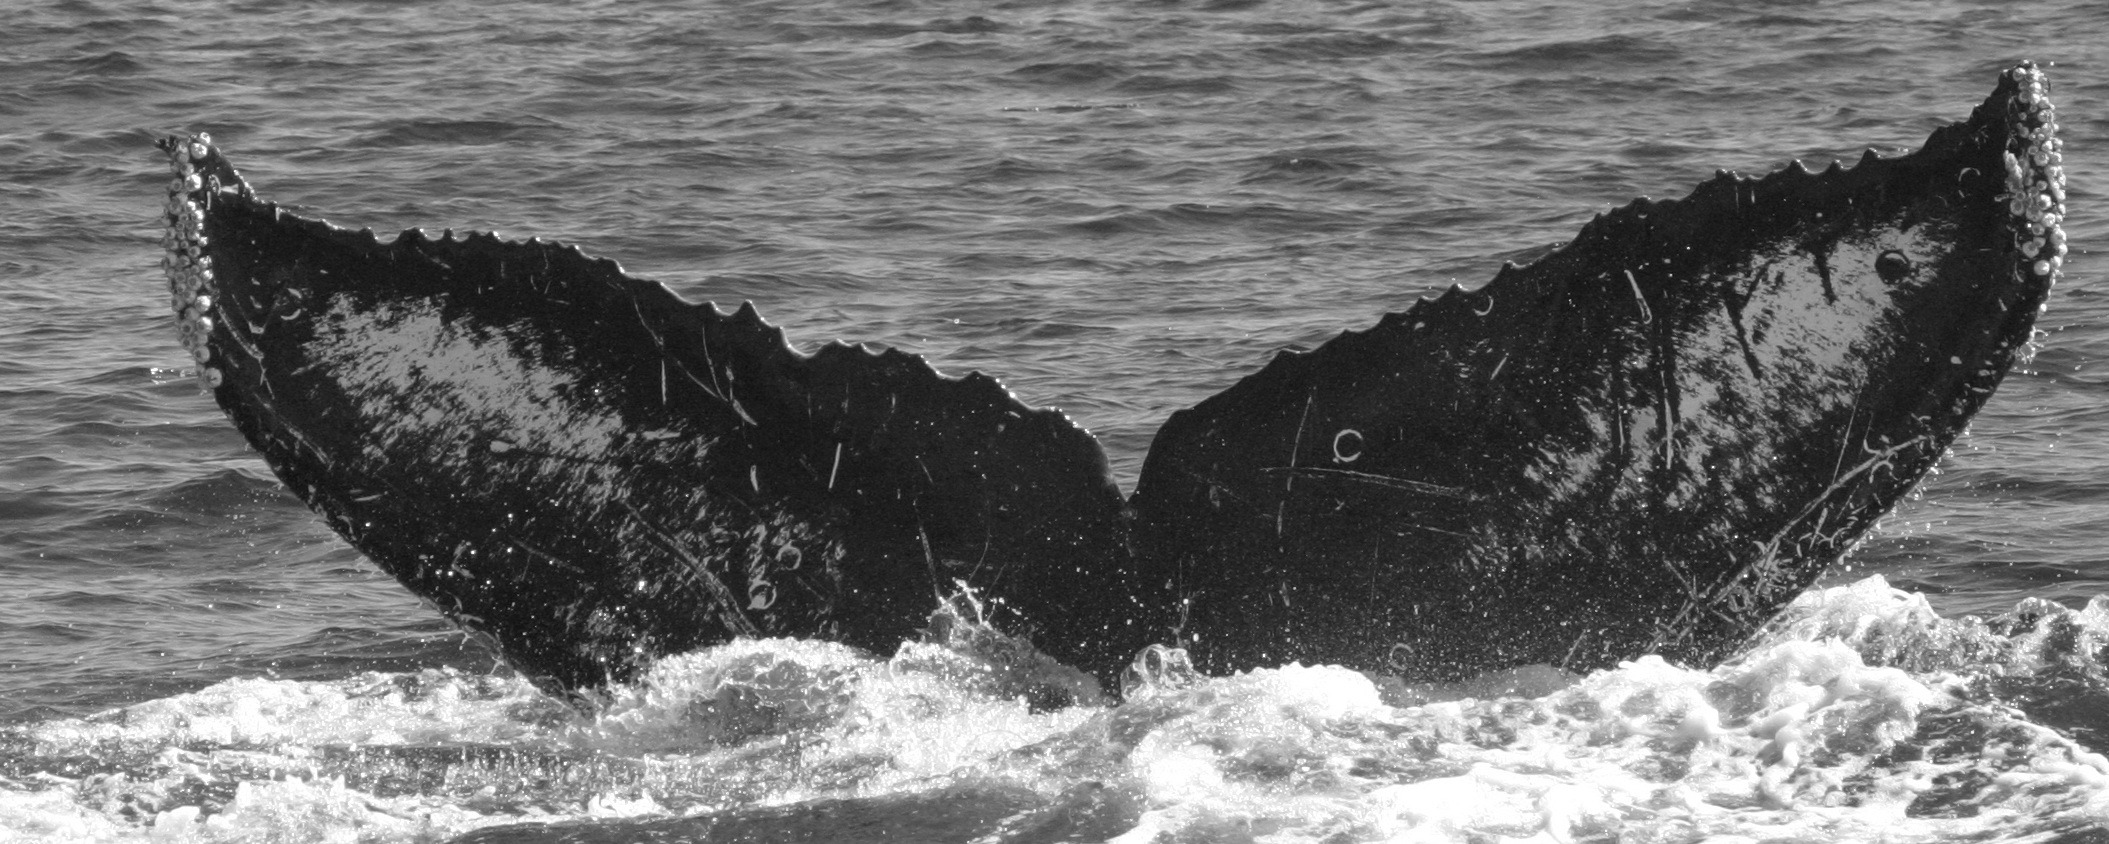
\includegraphics[width=1.0\textwidth]{../images/fluke_aid88_goodmatching.jpg}
\caption[]{\textbf{Example Fluke}. Example image of a humpback whale fluke from the SPLASH \cite{calambokidis2008splash} dataset \footnote{All images of humpbacks flukes in this thesis come from this dataset}. This image has a clearly visible trailing edge and internal fluke pattern.}
\label{fig:example_fluke}
\end{figure*}

\subsection{Distinguishing Individual Flukes}

The primary distinguishing features of these flukes are --- for the purposes of this work --- separated into two main areas; the ``trailing edge'' of the fluke, and the internal texture.
There are pros and cons to identification with either feature.
The internal texture is a more obvious choice for identification, as it is disinctive even from a distance and blurred, whereas trailing edges require high quality photographs.
However, there are humpback flukes who have indistinct (e.g.\ all-black) internal textures, which make matching based on texture impossible.
An example of this is shown in Figure \ref{fig:unclear_texture}.

Additionally, the work of Blackmer et al.\ \cite{blackmer2000temporal} finds that the trailing edge changes less with age than the internal texture of the fluke, which means that it can (potentially) be a more reliable identifier over time.

That said, the requirements for getting a good photograph of the trailing edge can be impractical, as the trailing edge can be obscured by out of plane rotations (an example is shown in Figure \ref{fig:unclear_te}).


\section{Current Identification Methods}

Computer-assisted photo-identification of humpback whale flukes has been attempted since the early 90s \cite{mizroch1990computer}.
While early efforts mostly relied on a manual description of the fluke that would then be matched (against other stored descriptions), later efforts have involved matching flukes based on automated analysis of both the internal texture and trailing edge.
\\\\
Existing computer-assisted photo-identification methods can be broadly separated into three categories:

\begin{itemize}
	\item Manually annotated -- a human must manually annotate or catalogue features on each fluke image, which are then automatically matched
	\item Semi-automated -- a human must guide an algorithm (e.g.\ by setting control points or highlighting interesting regions) that then automatically identifies the individual
	\item Fully-automated -- the algorithm can identify individuals from raw images
\end{itemize}

\begin{figure*}[t]%
\centering
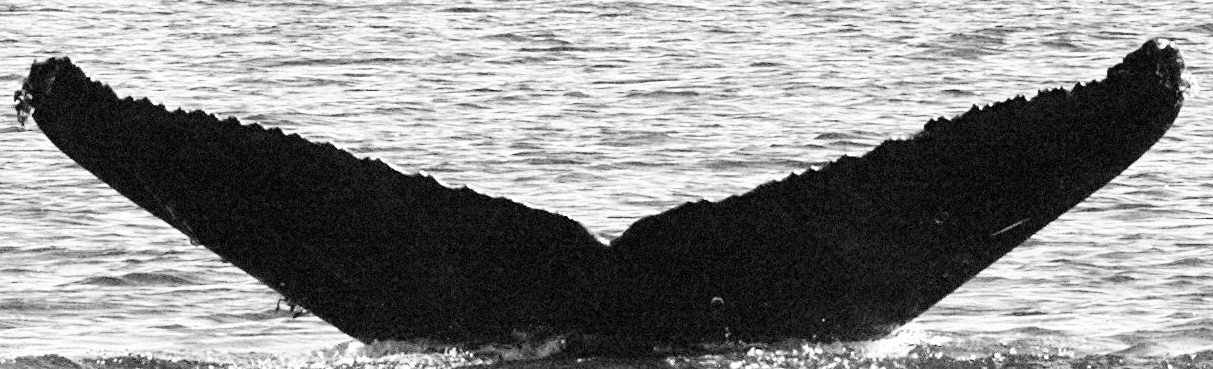
\includegraphics[width=1.0\textwidth]{../images/unclear_texture.jpg}
\caption[]{\textbf{Uniform Internal Texture}. This image of a humpback fluke shows no clear internal texture, but a distinctive trailing edge.}
\label{fig:unclear_texture}
\end{figure*}



\subsection{Based on Trailing Edge}

In the I3S contour system \cite{i3scontour}, the user must input start and end points on the query trailing edge, after which its contour is extracted.
This trailing edge is then resized and aligned so that it can be compared with absolute difference against the database trailing edges.
It also compares a set of possible shifts, rotations, and scales of the query trailing edge to account for these differences.
At the time of writing no published results on this system applied to humpback whales could be found.

Automatically identifying humpback whales by their entire trailing edge contour is done experimentally in Hughes et al.\ \cite{hughes2015automated}, using a technique that is originally designed for great white sharks. 
This technique segments the trailing edge into a set of possible contours and matches them combinatorially using Difference of Gaussians.
The authors achieve a comparable accuracy to our method, however for a much smaller dataset of humpback flukes than the one evaluated here.

While trailing edge matching has seen limited use in Humpback whale identification, it is a much more common technique in sperm whale (P.\ macrocephalus) identification \cite{huele2000finding}, \cite{beekmans2005comparison} \cite{whitehead1990computer}, with varying levels of manual effort.
We detail these methods below as the fluke trailing edge matching paradigm is similar across species.

In Whitehead's work \cite{whitehead1990computer}, points of interest on the trailing edge are entered and catalogued manually along with their positions.
In order to match these trailing edges, all of the points are compared, with a distance threshold.
This requires significant manual effort, and achieves a low accuracy \cite{beekmans2005comparison}.

To contrast, the method proposed by Huele et al.\ \cite{huele2000finding} uses a semi-automatic extraction of sperm whale trailing edge, and then applies wavelet transformations which are cross-correlated to determine a similarity measurement.

\begin{figure*}[t]%
\centering
\subfloat[][]{
	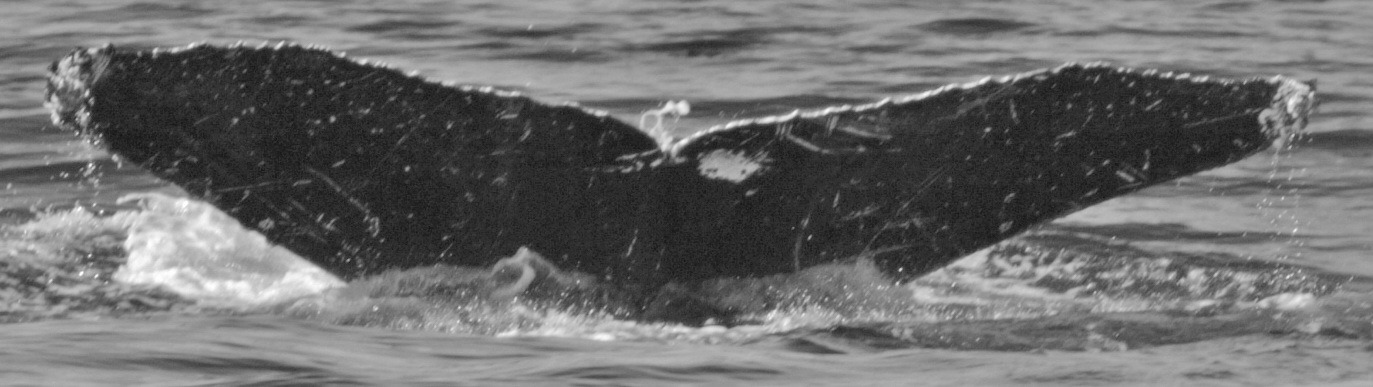
\includegraphics[width=1.0\textwidth]{../images/unclear_te_q.jpg}
}
\newline
\subfloat[][]{
	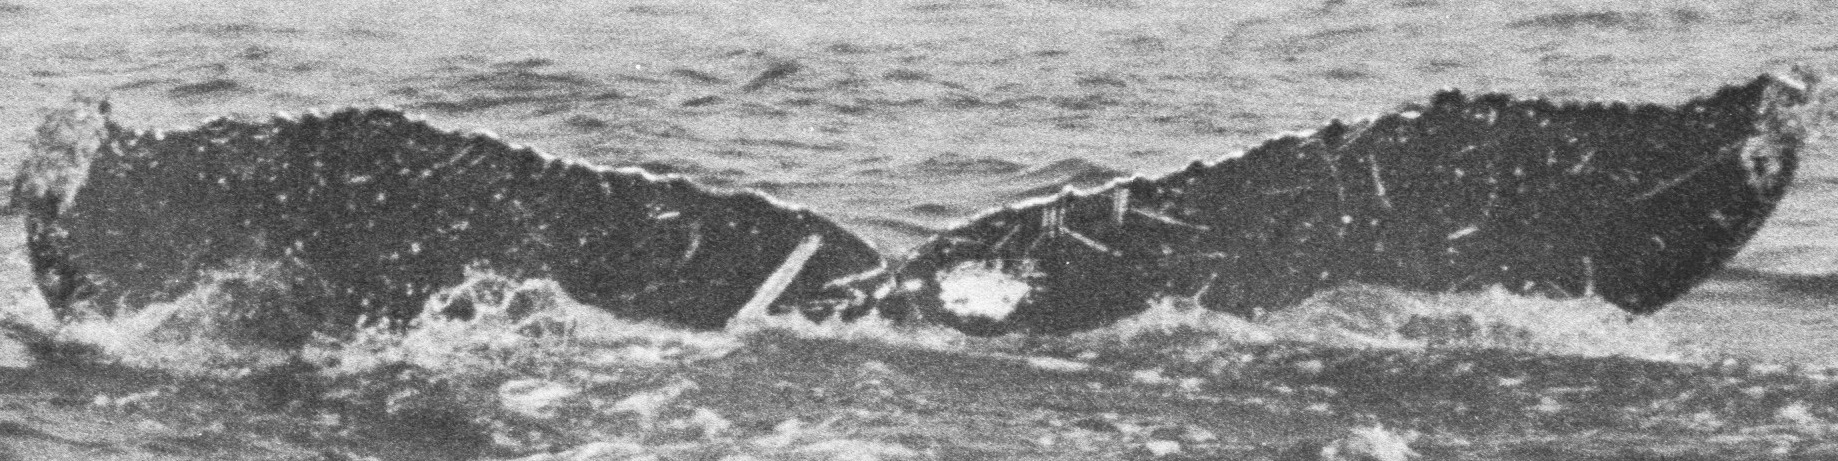
\includegraphics[width=1.0\textwidth]{../images/unclear_te_gt.jpg}
}
\caption[]{\textbf{Change in Trailing Edge}. The above images show that out of plane rotations of the fluke can obscure it or otherwise make it hard to match. These images are both of the same individual.}
\label{fig:unclear_te}
\end{figure*}

\subsection{Based on general Fluke appearance}


The primary method for computer-assisted photo-identification of humpback whale flukes is to use the internal fluke pattern, as seen in the work of Mizroch et al.\ \cite{mizroch1990computer} and Flukematcher \cite{kniest2010fluke}. 

In \cite{mizroch1990computer}, information about the fluke is manually catalogued and used to match individual whales. 
The fields that are catalogued contain information primarily about the overall coloration patterns of the fluke, as well as the shape of the central notch. 
The matching algorithm simply ranks flukes by looking at how similar annotated patterns are, and requires significant manual effort to identify individuals.

In Flukematcher \cite{kniest2010fluke}, control points (including the ones we use) are manually annotated which allow the program to automatically find pigmentation patterns in the fluke and align accordingly.
Optionally distinctive fluke patterns can also be selected by the user.
A variety of heuristic features are then extracted, which are matched using a variety of similarity measures.
This is an effective method, achieving 82\% top-1 accuracy on similar data to ours, but requires significant manual effort.

\section{Method Outline}

This method is, as stated before, a fully automated algorithm at test time, however in order to train the models some manual annotation is required.
The steps are roughly as follows, taking raw images as input.

\begin{itemize}
	\item Find the left and right tips of the fluke
	\item Extract the trailing edge contour betweeen these points
	\item Compute the curvature of the trailing edge contour at multiple scales
	\item Determine a ranking of possible identities using a distance computed by dynamic time warping 
\end{itemize}

We also combine this with a ranking from Hotspotter \cite{crall_hotspotter_2013}, a generalized appearance based identification method that has been successful for several different flukes. 

% TODO: Move this somewhere else?
%\subsubsection{Hotspotter}

%Hotspotter \cite{crall_hotspotter_2013} is an automated photo-identification algorithm based on SIFT features that has been used in identifying Grevy's zebras, plains zebras, giraffes, and several other species \cite{parham2015photographic}. 
%This work is the first to our knowledge that details Hotspotters efficacy when applied to Humpback whale flukes, and the results are presented in Chapter 4.
%That said, trailing edges are hard to photograph well, requiring high resolution imagery and a consistent angle between fluke and photographer.

%It should be noted that we used a segmenting convolutional network to aid Hotspotter's predictions, although this is not detailed in this work.

\section{The Dataset}

The main dataset that is used and evaluated in this work is a subset of the dataset collected by the SPLASH project \cite{calambokidis2008splash}. 
It consists of about 1400 identified photographs spread over about 860 identified individuals.
Of these, only 433 individuals have more than one image associated with them, giving 942 images that can be used in a one-to-one comparison.

We also use an external dataset of unidentified (but annotated) humpback flukes for training models.

\section{Thesis Outline}

The rest of this thesis will cover the background literature on many of the algorithms used in this work as well as the primary method itself.
We also detail some of the more significant alternatives that we evaluated, and how changing the various parameters of the main method affects identification accuracy.
We conclude with a discussion on the failings of the primary method, as well as ways to improve it and generalize it to identifying trailing edges in other animals.


%\section{Method Overview}

%The method for trailing edge identification put forth in this thesis is very nearly fully automated, requiring no human annotation when used (although manual annotation is necessary for training the machine learning models used).
%On its own, it achieves decent results on a (relatively) large dataset, comparable with the fully automated method used in \cite{hughes2015automated}. 
%Ultimately we find that this method is best used in combination with an automated pattern matching method (e.g. Hotspotter) to provide high accuracy matches.
%We also explore alternative methods based on more recent advances in deep learning for identification, however it appears that the dataset is too small to properly train these methods.


%%% Local Variables: 
%%% mode: latex
%%% TeX-master: t
%%% End: 
